\chapter{Cadre du projet}
\section*{Introduction}
\addcontentsline{toc}{section}{Introduction }
\par {\huge C}e chapitre introductif sera le départ pour la compréhension de notre projet. 
Nous commençons la première partie par le cadre et le contexte de notre projet. 
Ensuite, nous étudions les solutions existantes afin de cibler les insuffisances et l'embauche de notre nouvelle solution.
% Une section

% Exemple d'une section qui porte une référence à une bibliographie
% NB: il faut bien suivre le syntaxe pour ne pas tomber dans le cas où il y a une référence dans la table des matières.
\section{Context général du projet}
\par Ce projet Ce travail s'inscrit dans le cadre d'un sujet de fin d'études en vue de l'obtention du diplôme national d'ingénieur sein de L'\textbf{I}nstitut \textbf{S}upérieur de l'\textbf{I}nformatique \textbf{(ISI)}.
 Durant un stage de quatres mois effectués chez \textbf{Avaxia group}, notre mission consiste à concevoir et implémenter une platforme analytique pour les méta-données de la platforme Snowflake.
\section[Organisme d'accueil]{Organisme d'accueil}
\par Dans cette section, nous allons présenter l'organisme d'accueil \textbf{Avaxia Group}. 
\subsection{Présentation générale de Avaxia Group}

\par Avaxia Group, une entreprise de conseil en technologie créée en 1998 et ayant son siège à Dubaï, étend actuellement sa présence mondiale avec des bureaux  en Tunisie, au Japon et au Canada, et de futurs emplacements prévus en France et à Dakar. 
Avaxia Group se spécialise dans les solutions middleware, la gestion des infrastructures système, ainsi que dans le conseil fonctionnel, couvrant des domaines tels que l'architecture, l'intégration et les opérations \cite{avaxia}.
\subsection{Les services de Avaxia Group}
\par Avaxia Group opère sur le vaste marché international, avec une présence dans de nombreux pays. 
L'entreprise propose une gamme diversifiée de services, notamment les suivants\cite{serAvaxia}:

\setlist[itemize]{label=$\bullet$}
\begin{itemize}
\setlist[itemize]{label= \textbf{-}}

    \item \textbf{Expertise Technique en SAP: }
    \begin{itemize}
        \item  Gestion de l'infrastructure ;
        \item  Optimisation et amélioration des performances ;
        \item  Conception et architecture du paysage SAP ;
        \item  Installation des systèmes, configuration et mises à niveau ;
        \item  Assistance technique 24/7.
    \end{itemize}
    % 
    \item \textbf{Conseil Fonctionnel : }
            \begin{itemize}
                \item  Gestion fonctionnelle du déploiement et planification des tests ;
                \item  Conception de solutions métier pour le déploiement de nouveaux modules SAP.
        
            \end{itemize}
     \item \textbf{ Solutions Logicielles Personnalisées :}
            \begin{itemize}
                \item  Conception et développement de solutions logicielles utilisant des technologies telles que Java J2E, DELL BOOMI Flow, Salesforce et SAP Fiori.
            \end{itemize}
         \item \textbf{Intégration des Systèmes :}
            \begin{itemize}
                \item  Intégration de données et gestion des flux de données ;
                \item Intégration d'applications métier ;
                \item Développement et gestion d'API : DELL BOOMI, Atmosphère.
            \end{itemize}
    \item \textbf{Ingénierie des Données :}
            \begin{itemize}
                \item  Modélisation, découverte, traitement, visualisation et exploration des données, ainsi que gestion du Big Data.
            \end{itemize}
    \item \textbf{Nouvelles Technologies :}
            \par Création et déploiement de solutions logicielles d'entreprise en utilisant les dernières technologies, notamment :
            \begin{itemize}
                \item  Apprentissage automatique (Machine Learning) ;
                \item Réalité virtuelle (VR) ;
                \item Réalité augmentée (AR) ;
                \item Internet des objets (IoT).
            \end{itemize}
    
\end{itemize}
\par Cette gamme diversifiée de services reflète l'engagement d'Avaxia Group à fournir des solutions techniques avancées et à rester à la pointe de l'innovation pour répondre aux besoins variés de ses clients à l'échelle mondiale.


\section{\'Etude du projet}
\par Dans cette section, nous explorons en détail l'étude de ce projet toutes en commmançant par la problématique qui a menée à sa réalisation,et les spécifications de cette derniére ainsi que son objectif.
\subsection{Problématique}
\par Avec l'avènement des technologies de cloud computing et des entrepôts de données modernes tels que Snowflake, les entreprises disposent désormais d'une flexibilité 
et d'une évolutivité inégalées pour la gestion et l'analyse de leurs données. 
Cependant, cette transition vers le cloud présente des défis spécifiques en termes de performance, de coûts, et de surveillance des opérations. 
\par Dans ce contexte, Avaxia Group ainsi que ces clients, se trouvent confronter à des problématiques particulières liées à l'utilisation de Snowflake, leurs entrepôt de données principal, telque : 
\begin{itemize}
    \item \textbf{Gestion des performances : } \par - Avaxia Group constate des délais dans l'exécution des requêtes et des temps de traitement prolongés lors de l'utilisation de Snowflake. 
    Ces problèmes impactent directement la productivité des équipes et la satisfaction des utilisateurs finaux ;

    \par - les requêtes \textbf{S}tructured \textbf{Q}uery \textbf{L}anguage \textbf{(SQL)} complexes ou mal optimisées peuvent engendrer des goulets d'étranglement et des inefficacités dans l'utilisation des ressources de Snowflake, du coup elles
    nécessitent une surveillance et une optimisation constantes ;

    \item \textbf{Maîtrise des coûts :} \par - les coûts associés à l'utilisation de Snowflake peuvent rapidement augmenter en raison d'une gestion inadéquate des ressources. 
    Avaxia Group doit donc trouver des moyens de maîtriser les coûts tout en garantissant des performances optimales pour ses opérations ;

    \item \textbf{Surveillance et analyse des opération :} \par - pour assurer le bon fonctionnement de ses opérations Snowflake, Avaxia Group a besoin d'une solution de surveillance avancée pour détecter les anomalies, identifier les goulets d'étranglement et optimiser les performances.
    \par De plus, une analyse approfondie des métriques opérationnelles telles que le temps d'exécution des requêtes, l'utilisation des ressources et les performances des entrepôts sont essentielles pour optimiser l'efficacité et l'efficience des opérations. 
\end{itemize}

\subsection{Analyse et critique de l'existant}
Dans cette section, nous passerons en revue les fonctionnalités, les avantages de chaque solution existante, tout en mettant en lumière les lacunes qui ont conduit au développement de notre propre solution de monitoring des opérations Snowflake.
\subsubsection{Analyse de l'existant}
\par L'analyse de l'existant est une étape cruciale dans le processus de développement de notre solution.
C'est pour céla, nous allons entammer l'analyse les outils existants utilisés pour surveiller et analyser les opérations sur les divers plateformes de l'analyse des données et le cloud data warehousing.
\begin{itemize}
    \item\textbf{Snowflake account usage dashboard :}  est un tableau de bord intégré dans snowflake qui fournit des informations sur l'utilisation de Snowflake, telles que le nombre de sessions utilisateur, 
    la quantité de données stockées et le temps \textbf{C}entral \textbf{P}rocessing \textbf{U}nit (\textbf{CPU}) utilisé.
    Il offre une vue rétrospective des opérations passées, permettant aux utilisateurs de comprendre l'historique d'utilisation de la plateforme. 
    \par La figure \textbf{\ref{fig:SAU}} suivante illustre une partie de cette dashboard:
        %code image
            \begin{figure}[H]
            \centering
            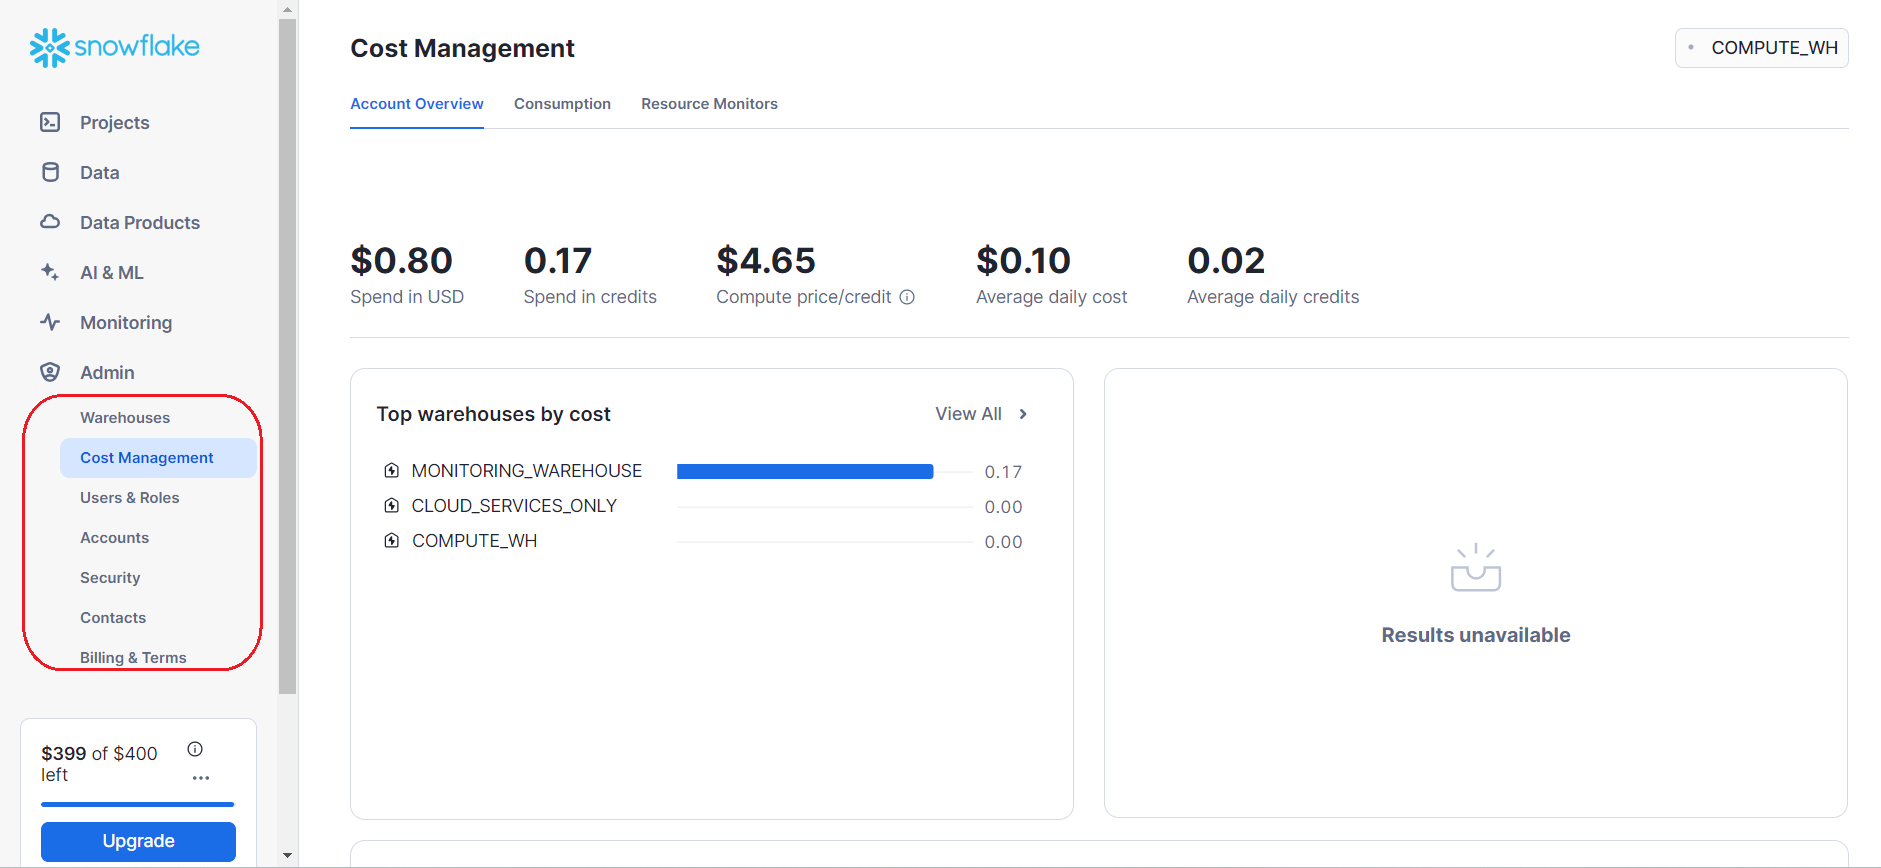
\includegraphics[width =13cm, height=7.5cm]{img/captures/account_usage}
            \caption{Snowflake account usage dashboard}
            \label{fig:SAU}
            \end{figure}
        %fin
    \item\textbf{Snowflake Information Schema :} est une collection de vues système qui fournissent des métadonnées sur les objets et les opérations effectuées dans un compte Snowflake. 
    Ces vues offrent une granularité élevée pour examiner les détails des requêtes SQL exécutées, les performances des entrepôts de données et d'autres aspects des opérations Snowflake. 
    \par La figure \textbf{\ref{fig:info}} suivante illustre une partie de cette vue:
        %code image
            \begin{figure}[H]
            \centering
            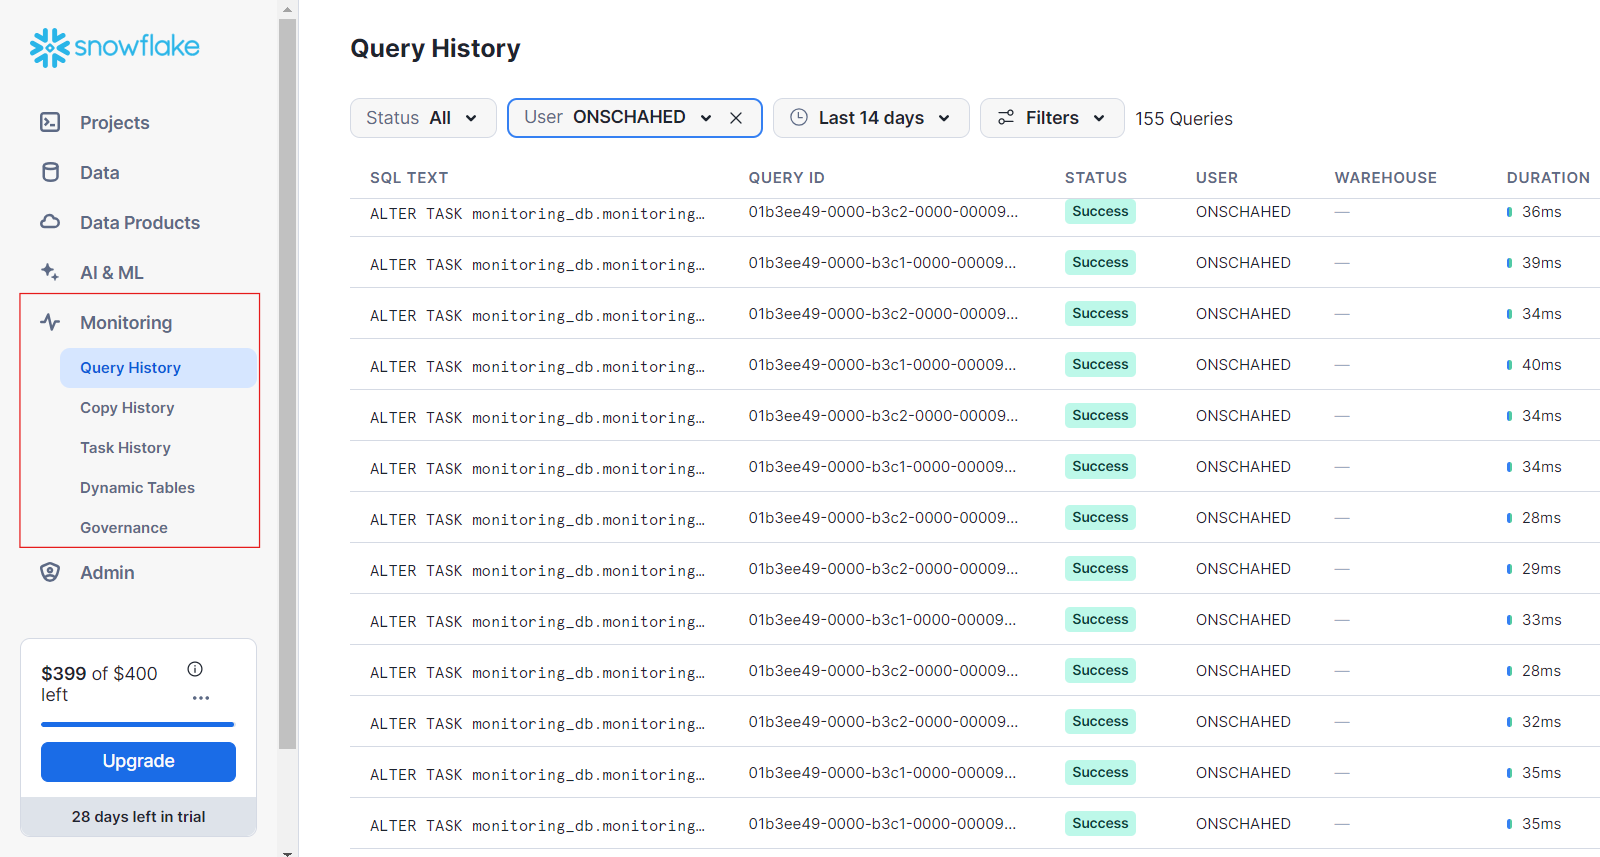
\includegraphics[width =13cm, height=7.5cm]{img/captures/info}
            \caption{Snowflake account usage dashboard}
            \label{fig:info}
            \end{figure}
        %fin
    \item\textbf{Google BigQuery :} est une autre option populaire pour le stockage et l'analyse des données dans le cloud. 
    Il offre des fonctionnalités avancées telles que le traitement massivement parallèle et la capacité à exécuter des requêtes SQL complexes sur de grands ensembles de données. 
    \par La figure \textbf{\ref{fig:BQ}} suivante illustre une partie de tableau de bord de BigQuery :
        %code image
            \begin{figure}[H]
            \centering
            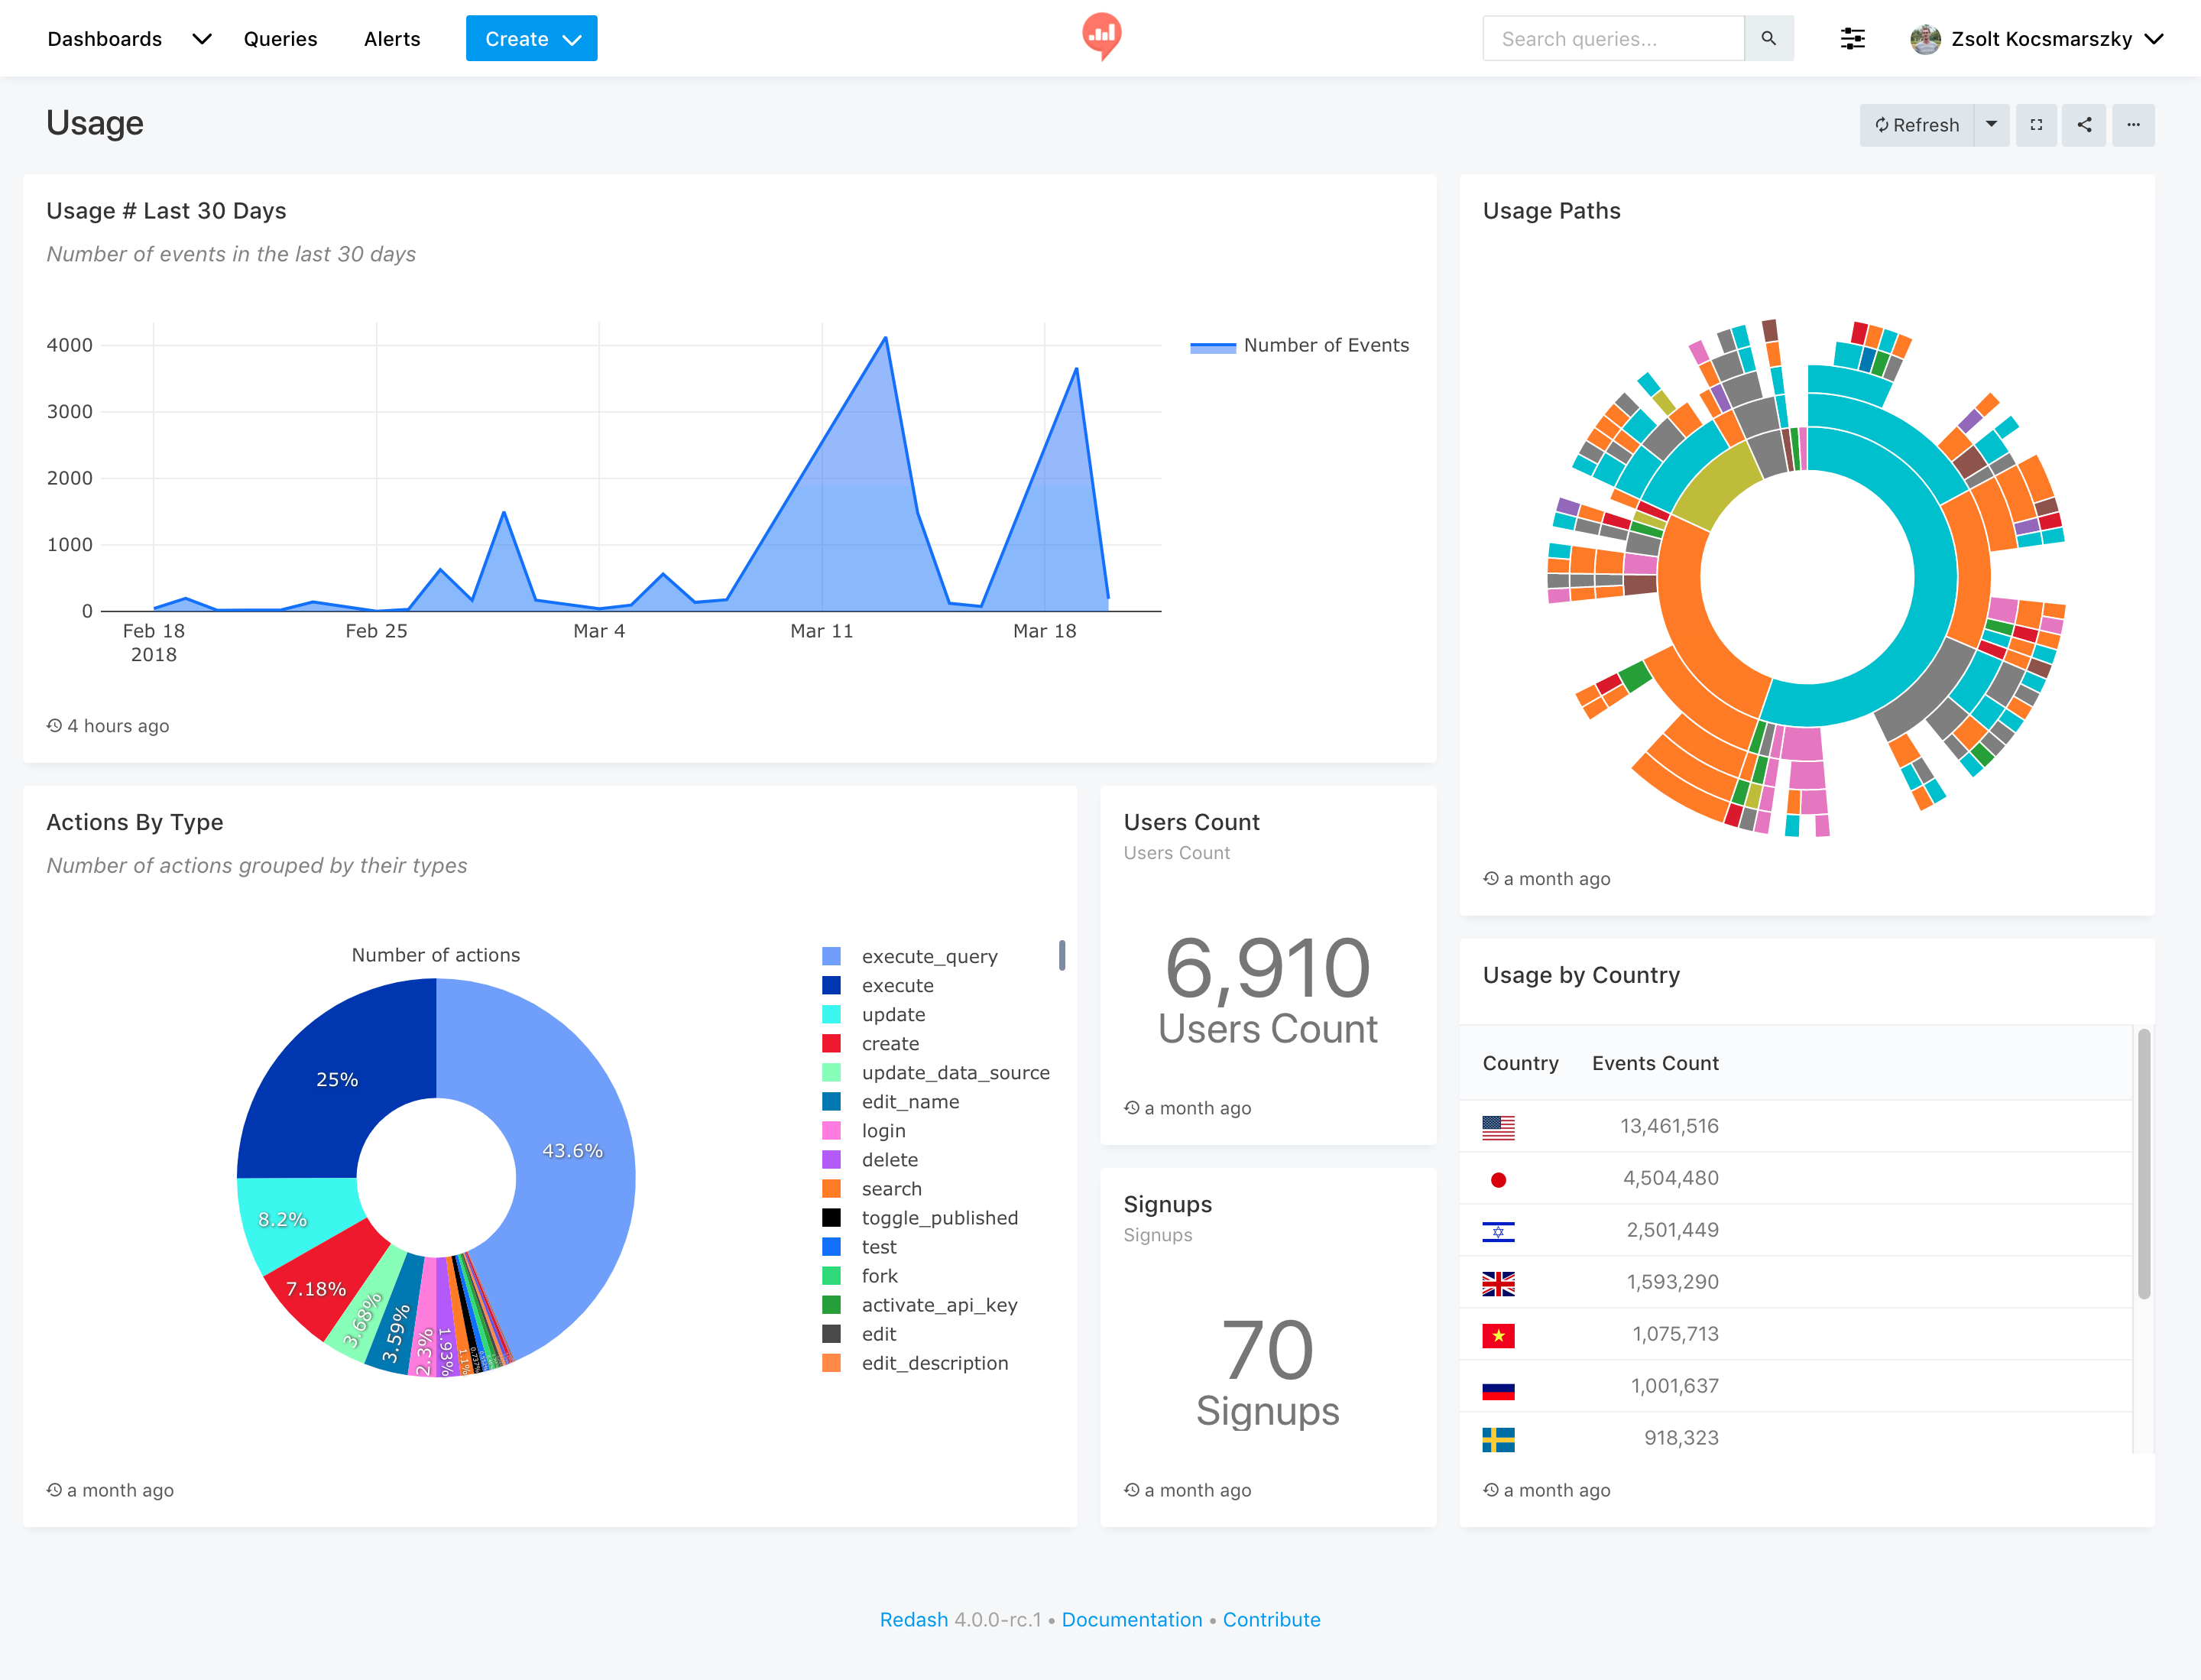
\includegraphics[width =13cm, height=7.5cm]{img/captures/bigquery}
            \caption{Tableau de bord de <<Google BigQuery>>}
            \label{fig:BQ}
            \end{figure}
        %fin

    \item\textbf{Amazon Redshift :} est un entrepôt de données cloud basé sur PostgreSQL, conçu pour gérer de gros volumes de données et exécuter des analyses complexes.
    Il offre des performances élevées et une extensibilité, mais son modèle de tarification basé sur l'utilisation des ressources peut entraîner des coûts supplémentaires pour les entreprises.
    \par La figure \textbf{\ref{fig:RS}} suivante illustre le tableau de bord de ResShift:
        %code image
            \begin{figure}[H]
            \centering
            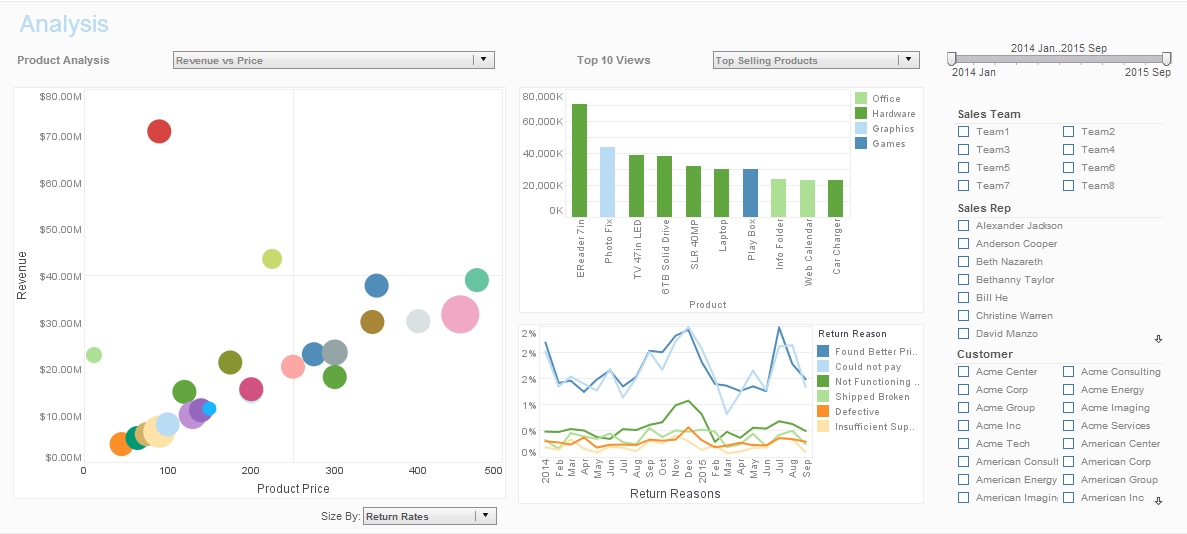
\includegraphics[width =13cm, height=7.5cm]{img/captures/redshift}
            \caption{Tableau de bord de "Amazon Redshift"}
            \label{fig:RS}
            \end{figure}
        %fin
\end{itemize}
\subsubsection{Critique de l'existant}
\par Dans cette section, nous allons examiner de manière critique les solutions actuellement utilisés dans le domaine de l'analyse de données, afin de fournir une base solide pour concevoir une solution qui surmonte les limitations et offre une valeur ajoutée significative à nos parties prenantes.
\begin{itemize}
    \item\textbf{Complexité des solutions : }les solutions de surveillance existants, comme le Snowflake Information Schema, sont souvent complexes à utiliser et nécessitent des compétences techniques avancées pour interpréter les données fournies. 
    Cette complexité peut rendre difficile la compréhension des métriques et la prise de décisions éclairées par les équipes opérationnelles ;
    (par exemple dans un flux de travail si une certaine tache est échouée, les indicateurs disponibles sur snowflake ne peuvent pas identifier ou exactement le workflow est suspendu de façon à rendre les choses plus compliqué pour les utilisaturs de Snowflake de détecter les anomalies si ils savent pas comment le manipuler techniquement.)

    \item\textbf{Personnalisation limitée : }les options de personnalisation offertes par les outils existants sont souvent limitées. 
    Par exemple, Google BigQuery propose des fonctionnalités avancées, mais la personnalisation des tableaux de bord et des rapports est restreinte. Cela peut être un obstacle pour les entreprises ayant des besoins spécifiques en matière de surveillance et d'analyse des performances ;

    \item\textbf{Coûts supplémentaires : }certains outils, comme Amazon Redshift, peuvent entraîner des coûts supplémentaires importants pour les entreprises. La tarification basée sur l'utilisation des ressources peut rapidement augmenter, surtout si les entreprises ne surveillent pas activement leur utilisation. Cela peut constituer une barrière financière pour les petites et moyennes entreprises souhaitant utiliser ces outils de surveillance ;

\end{itemize}

\subsection{Objectif du projet}
\par  L'objectif principal de ce projet est de propulser les opérations Snowflake d'Avaxia Group vers de nouveaux sommets en termes de performance, de rentabilité et d'efficacité. 
Le développement de cette nouvelle plateforme de surveillance aidera l'équipe d'Avaxia à surmonter ces défis majeurs.
\par Grâce à cette initiative, Avaxia Group pourra optimiser ses processus, réduire les coûts opérationnels et améliorer la qualité des services offerts à ses clients. En effet, cette nouvelle plateforme 
permettra de détecter rapidement les problèmes de performance, d'anticiper les besoins en ressources et de garantir une gestion plus efficace des opérations.
\subsection{Solution proposée}
\par Notre solution repose sur la conception et l'implémentation d'un système de surveillance et d'optimisation des opérations exhaustif. 
Cette solution se repartie en plusieurs composants clés, chacun ciblant des aspects spécifiques des problématiques identifiées:

\begin{itemize}
    \item La mise en place des stratégies de monitoring en temps réel cela permettra d'identifier rapidement les problèmes de performance et de prendre des mesures correctives efficaces ;
    \item le développement d'outils d'analyse avancée des coûts qui aiderent nos utilisateurs finaux à mieux comprendre ses dépenses et à trouver des opportunités d'optimisation pour 
    réduire les coûts tout en maintenant des performances élevées ;
    \item Développement des tableaux de bord interactifs et riches en informations pour permettre à Avaxia Group et à ses clients de surveiller en temps réel les performances de leurs opérations Snowflake. 
    Ces tableaux de bord fourniront des indicateurs clés de performance, des graphiques et des visualisations pour faciliter la détection des anomalies et la prise de décisions éclairées ;
    \item Utilisation de techniques d'analyse avancée des données opérationnelles pour permettre aux utilisateurs  d'identifier les opportunités d'amélioration et d'optimisation de leurs opérations, 
    renforçant ainsi leur compétitivité et leur efficacité ;
    \item Développement d'algorithmes d'optimisation des requêtes SQL afin de de réduire les temps d'exécution et de minimiser les goulets d'étranglement dans l'utilisation des ressources de Snowflake.
\end{itemize}


\section{Choix méthodologique}
\par Dans le but d'aboutir à une solution de qualité qui répond aux besoins exigés dans des
temps et des coûts prévisibles, le choix du processus de développement convenable est
une phase primordiale dans tout projet. Nous devons appliquer une méthode rigoureuse
sur la conduite de notre projet.
\subsection{Différence entre Scrum et Kanban}
\par La table \textbf{1.1} résume une comparaison entre les méthodes agiles de gestion des projets \textbf{Scrum} et \textbf{Kanban} :
\begin{table}[H]
    \centering
    \begin{tabular}{|p{3.5cm}|p{6cm}|p{6cm}|}
        \hline
        \rowcolor{blue!18}\textbf{\hbox{Point de comparaison}} & \textbf{Scrum} & \textbf{Kanban} \\
        \hline
        \textbf{Origine} & Développement logiciel & \hbox{ Fabrication Lean (Lean Manufacturing)} \\
        \hline
        \textbf{Idéologie} & Apprendre de ses expériences,\par s'organiser et hiérarchiser, et réfléchir à ses réussites et ses échecs afin de s'améliorer en permanence & Utiliser des visuels pour améliorer le travail en cours \\
        \hline
        \textbf{Cadence} & Sprints réguliers et à durée déterminée (à savoir, deux semaines) & Flux continu \\
        \hline
        \textbf{Bonnes pratiques }& Planification du sprint, sprint, mêlée \par quotidienne (Daily Scrum), revue du sprint, rétrospective du sprint & Visualiser le flux de travail, limiter le travail en cours, gérer le flux, intégrer des boucles de rétroaction \\
        \hline
        \textbf{Rôles }& Product Owner, Scrum Master, équipe de développement & Aucun rôle requis \\
        \hline
        \textbf{Utilisation des tableaux} & Un tableau Scrum est nettoyé et recyclé après chaque sprint & Un tableau Kanban est utilisé tout au long du cycle de vie d'un projet \\
        \hline
        \textbf{Nombre des tâches }& Un tableau Scrum possède un nombre \par de tâches définies ainsi que des\par échéances strictes pour les effectuer&
        Les tableaux Kanban sont plus flexibles en termes de tâches et d'échéances. Les tâches peuvent être hiérarchisées à nouveau, réassignées ou mises à jour si besoin. \\
        \hline
       
    \end{tabular}
    \label{tab:difference}
\caption{Comparaison entre les méthodes de gestion du projet Scrum et Kanban }
\end{table}

\subsection{Justification de choix}
\par Notre choix de Kanban comme étant pour la gestion de notre projet est le fruit d'une réflexion stratégique minutieuse. 
En effet, Kanban, qui tire son origine du terme japonais signifiant << tableau >>\cite{origine}, se démarque par sa flexibilité, sa transparence et sa focalisation sur l'amélioration constante.

\par Dans le cadre de notre projet, Kanban s'impose naturellement comme le choix optimal. 
Cette méthode permet une gestion visuelle et en temps réel des tâches et des flux de travail, une caractéristique cruciale pour un projet centré sur l'analyse de données et la visualisation.
 Chaque étape de notre processus, de la collecte des données à la présentation des résultats, trouve une représentation claire et concise dans le tableau Kanban.

\par De surcroît, Kanban promeut une approche itérative et progressive, parfaitement en harmonie avec notre objectif d'amélioration continue. 
Elle autorise une gestion fluide et adaptable des tâches, offrant la souplesse nécessaire pour ajuster notre plan en fonction des découvertes et des besoins changeants du projet.
\par En optant pour Kanban, nous mettons l'accent sur la transparence et la communication au sein de l'équipe. 
Chacun dispose d'une vision limpide de l'état d'avancement du projet, favorisant ainsi la collaboration et l'engagement de tous les membres.
\subsection{Le tableau Kanban}
\par Un tableau Kanban est un outil de gestion de projet Agile conçu pour aider à visualiser le travail, limiter le travail en cours et maximiser l'efficacité (ou le flux) \cite{kanban}.
\par Dans cette section, nous allons s'interésser à la spécificités des tableaux Kanban et leurs types

\subsubsection{Composants d'un tableau Kanban}
\par Dans cette partie, nous allons découvrir les composants d'un tableau Kanban. En effect, Les tableaux Kanban utilisent des cartes, des colonnes, des couloirs et des limites de travail 
en cours pour permettre aux équipes de visualiser et de gérer efficacement leurs flux de travail. Examinons ces principaux éléments plus en détail:

\begin{itemize}
    \item{\textbf{Carte Kanban}} : c'est une représentation visuelle des tâches. Chaque carte contient des informations importantes sur la tâche, telles que sa description, son statut d'avancement, les personnes impliquées, 
    les échéances, etc\cite{tableau} ;
    \item {\textbf{Colonne Kanban}}:chaque colonne une étape distincte du processus de travail. Les tâches traversent ces différentes colonnes au fur et à mesure 
    de leur avancement, jusqu'à ce qu'elles soient complètement terminées. Cette organisation visuelle permet de suivre et de maîtriser le flux de travail de manière efficace \cite{tableau} ;

    \item{\textbf{Couloir Kanban}} : sont des bandes horizontales pour séparer différents éléments tels que les activités, les équipes, les classes de service, etc.
     Ces bandes permettent d'organiser visuellement le tableau de manière plus granulaire et de mieux différencier les éléments qui le composent \cite{tableau} ;

     \item{\textbf{Limite de travail en cours}} : elles limitent la quantité maximum de tâches dans les différentes étapes du flux de travail.
      Elles vous permettent de terminer des tâches plus rapidement en aidant votre équipe à ne concentrer que sur les tâches en cours \cite{tableau};

    \item{\textbf{Point d'engagement}} : un point d'engagement est un point dans le processus de travail auquel une tâche est prête à être incorporée au système \cite{tableau} ;
    \item{\textbf{Point de livraison }} : point du flux de travail auquel une tâche est considérée comme terminée \cite{tableau}.
\end{itemize}
    \subsubsection{Types des tableaux Kanban}
    \par Les tableaux Kanban peuvent être divisés en plusiedeux types :
    \begin{enumerate}
        \item[1-]\textbf{Un tableau Kanban physique }: est la forme la plus basique, les équipes utilisent des Post-its (représentant des tâches) et un tableau blanc (ou en liège). 
        Les phases de travail sont représentées par des colonnes et les Post-its sont déplacés d'une étape à une autre \cite{tableau}.
        \item[2-]\textbf{Un tableau Kanban numérique }: est une solution logicielle, ce qui le rend plus accessible que son pendant physique. Il peut vous fournir une visibilité sur la progression du travail depuis quasiment n'importe où, ce qui facilite la collaboration d'équipe. 
        Certaines solutions numériques s'avèrent très souples, permettant aux responsables de suivre plusieurs flux de travail et d'organiser leur travail en différentes catégories \cite{tableau}.
    \end{enumerate}
\par Pour la gestion de notre projet, nous avons choisi \textbf{<< Trello >>} qui est une platforme rapide et simple pour la création d'un tableau Kanban numérique.


\par En résumé, la méthode Kanban s'impose comme un choix stratégique judicieux pour notre projet, offrant un cadre solide pour une gestion efficace, transparente et itérative, tout en servant l'objectif fondamental d'amélioration continue de la performance de l'équipe.

\section*{Conclusion}
\addcontentsline{toc}{section}{Conclusion}
   À la clôture de ce chapitre initial, nous avons jeté les fondements pour la compréhension complète de la sphère du projet. Cette phase est cruciale pour cadrer les enjeux et les perspectives qui guident notre travail. Dans le prochain chapitre, nous explorerons en détail l'analyse et la spécification des besoins, une étape essentielle pour la réalisation de notre projet.